\documentclass[10pt]{article}
\usepackage{parskip}
\usepackage[utf8]{inputenc}
\usepackage[left=2.00cm, right=2.00cm, top=2.00cm, bottom=2.00cm]{geometry}
\usepackage[spanish]{babel}
\usepackage{graphicx,subfig}
\usepackage{fancyhdr}
\usepackage{pgfplots}

\graphicspath{{Imagenes/}}
\usepackage{enumerate} 
\usepackage{multicol}
\usepackage{tabularx}
\usepackage{amssymb}
\usepackage{adjustbox}
\usepackage{amsmath}
\usepackage{cancel}
\begin{document}


\pagestyle{fancy}
\cfoot{}


%Cabeceras
\rhead{Ley de Ohm.}
\lhead{}

%Portada
\begin{titlepage}
	\newgeometry{
		left=25mm,
		right=25mm,
		top=5mm,
		bottom=30mm,
		headheight = 0 mm
	}

	\begin{figure}[t]
		\subfloat{
\includegraphics[width=0.15\textwidth]{Logo_IPN}}
		\hspace{0.6\textwidth}
		\subfloat{
\includegraphics[width=0.22\textwidth]{LogoEsime}}
	\end{figure}

	\centering
	{\bfseries\Huge Instituto Politécnico Nacional. \par}
	\vspace{1cm}
	{\scshape\Large Ingeniería en Comunicaciones y Electrónica. \par}
	\vspace{0.3cm}
	{\scshape\Large Laboratorio de Electricidad y Magnetismo.  \par}
	\vspace{1cm}
	{\scshape\Huge Victoria la Reina Insaciable \par}
	\vspace{1cm}
	{\itshape\Large Ley de Ohm. \par}
	{\Large 2CM13\par}
	\vfill
	{\Large Autores: \par}
	{\Large Daniela Elizabeth Pérez Vargas. \par}
	{\Large Jesús Martinez Amac. \par}
	{\Large José Emilio Hernández Huerta. \par}
	{\Large Nataly Bejarano Garduño.\par}
	{\Large Uriel Grimaldi Díaz.  \par}
	\vfill
	{\Large Junio 2023. \par}

\end{titlepage}

\tableofcontents
\newpage

\section{Resumen.}
En la practica con el material especifico comprobamos la ley de ohm midiendo desde el potencial electrico como la intensidad mediante un circuito en serie el cual regulamos con una caja especial con la cual podemos variar la recistencia que esta experimenta y tambien con un switch integrado en el circuito para hacer más facil el cambio en la funte de alimentacion terminando con la tabulacion de los resultados. 

\begin{multicols}{2}

\section{Objetivo.}
Se verificara que la corriente en un resistor ohmico es directamente proporcional a la diferencia de potencial entre sus bornes, dentro de los limites de precision del experimento, tambien establecera la relacion matematica entre la resistencia de un resistor ohmico y la corriente que lo atraviesa cuando el voltaje permanece constante y vericaran el comportamiento del circuito al variar la resistencia y el voltaje para mantener la corriente constante.


\section{Introducción.}
En nuestra formacion como ingenieros electronicos necesitaremos las bases para comprender, analizar, crear, reparar y entre muchos más, sistemsas electronicos pero para esto es sumamnete necesaria la ley de Ohm la cual establece que la diferencia de potencial que aplicamos entre los extremos de un conductor determinado es proporcional a la intensidad de la corriente que circula por el citado conductor.
Aunque esto parezca innecesario las practicas de laboratorio son importantes pues como en la vida laborar si aqui nos equivocamos quemando algun material tendremos consecuencia pero mientras que afuera seria un despido aqui solo es reponer el material y en tu calificacion, asi que le doy animos a cualquiera que lea este reporte.


\section{Marco teórico.}

La ley de Ohm establece una relación directa y proporcionalidad entre la corriente eléctrica y la diferencia de potencial (voltaje) en un circuito eléctrico cerrado (1)(2). En su forma más básica, la ley de Ohm establece que la corriente que fluye a través de un conductor es igual a la diferencia de voltaje entre los extremos del mismo (2)(3) , dividida por la resistencia del conductor:
$I = V/R$
Donde I es la corriente en amperios, V es la diferencia de voltaje en voltios (3) y R es la resistencia eléctrica del conductor en ohmios. Por lo tanto, la corriente y el voltaje están estrechamente relacionados en un circuito eléctrico. Además, la ley de Ohm también puede usarse para calcular la resistencia eléctrica de un conductor (2) diferencia de voltaje necesaria para producir una corriente determinada (3) o la corriente que fluirá en un circuito de resistencia determinada a partir de una diferencia de voltaje conocida.
\begin{center}
	
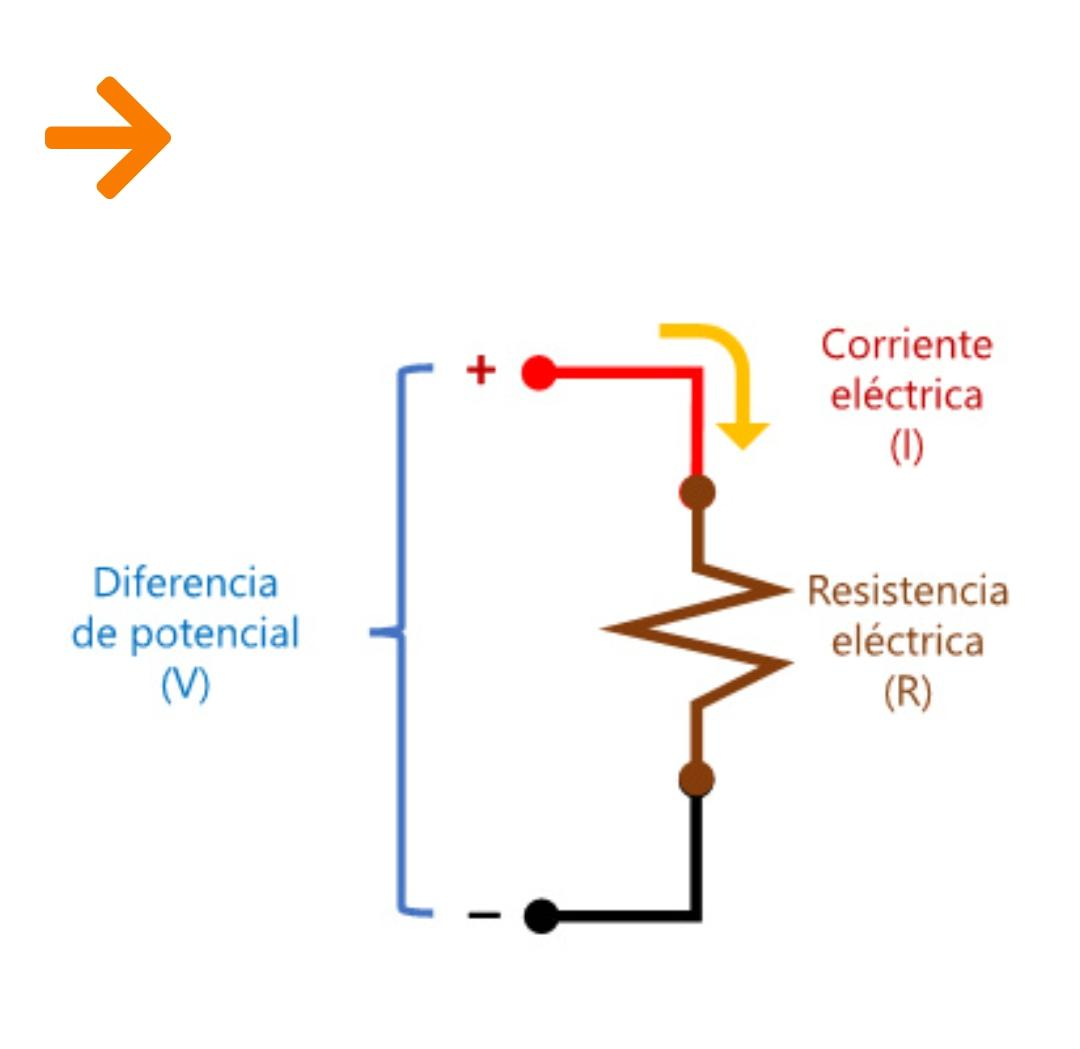
\includegraphics[width=0.17\textwidth]{lol}\\
Circuito Electrico \newline
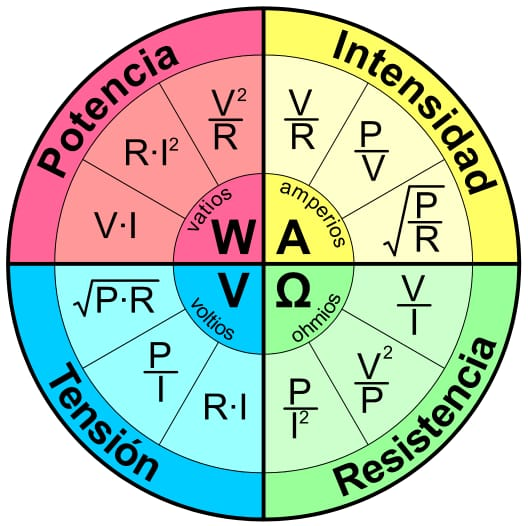
\includegraphics[width=0.17\textwidth]{reina}\\
Formulas para ley de Ohm

\end{center}
\section{Descripción de materiales.}

\subsection{Multimetro digital.}

Un multímetro digital es una herramienta que nos permite medir diferentes magnitudes eléctricas como voltaje, corriente y resistencia. A diferencia de los multímetros analógicos, los digitales tienen una pantalla en la que se muestra el valor medido. También pueden medir continuidad, capacitancia, frecuencia y temperatura. Son ampliamente utilizados en reparaciones y mantenimiento de circuitos electrónicos, así como en instalaciones eléctricas.

\begin{center}
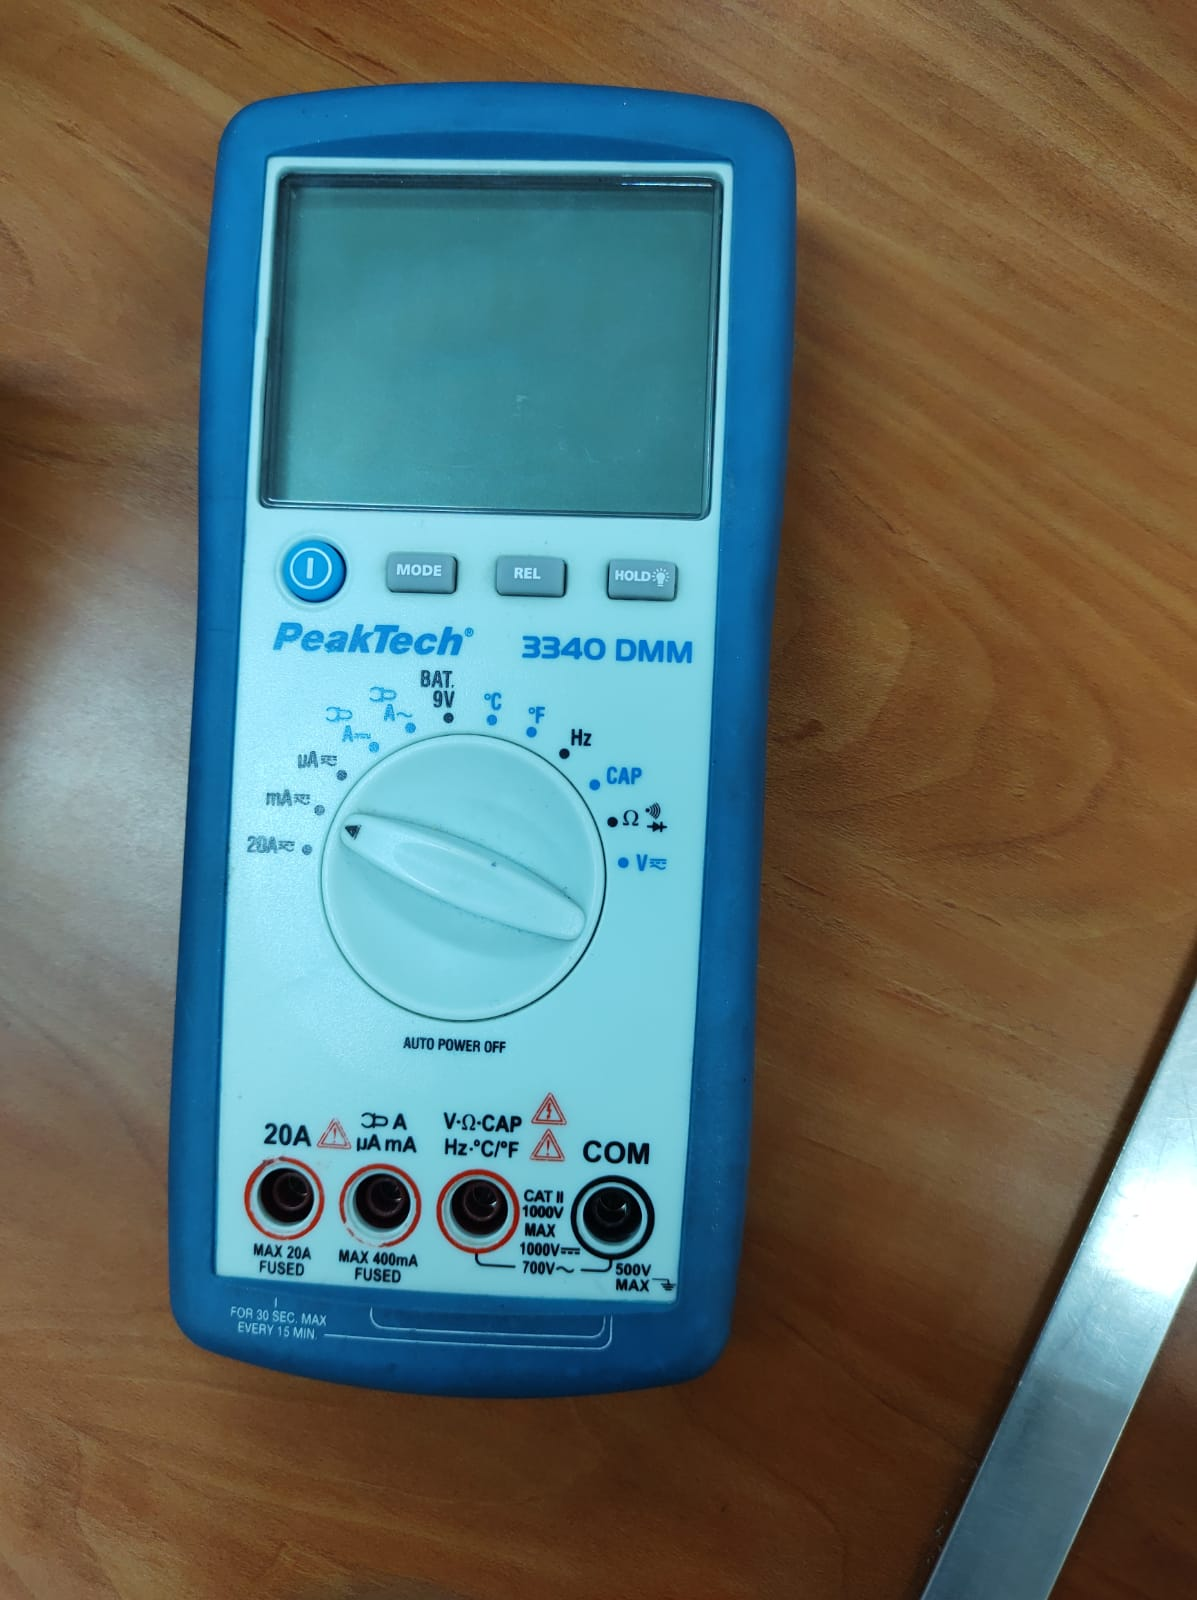
\includegraphics[scale=0.1]{Multimetro}\\
Reconocimiento del Multimetro digital.
\begin{enumerate}
\item La maraca del Multimetro es PeakTech.
\item Es un miltimetro digital de 3340 DMM.
\item Cuenta con 4 botones, el de encender, el mode, el rel y el hold.
\item Cuenta con 12 posiciones en la perilla de AUTO POWER OFF.
\item Cuenta con una terminal de entrada negativa.
\item Cuenta con 3 terminales de entradas positivas.
\end{enumerate}
\end{center}

\subsection{Selector bipolar.}

Un selector bipolar es un interruptor eléctrico que permite elegir entre dos opciones mediante la conexión o desconexión de dos terminales, los cuales están polarizados de forma opuesta entre sí. Por lo general, un selector bipolar tiene dos pares de terminales o polos, cada uno con su propio conjunto de contactos. Al activar uno de los conjuntos de contactos, se cierra ese circuito y se abre el otro, permitiendo que la corriente fluya a través del circuito seleccionado. Es comúnmente utilizado en aplicaciones eléctricas donde se requiere conmutación de señales, como en equipos de audio y amplificadores.

\begin{center}
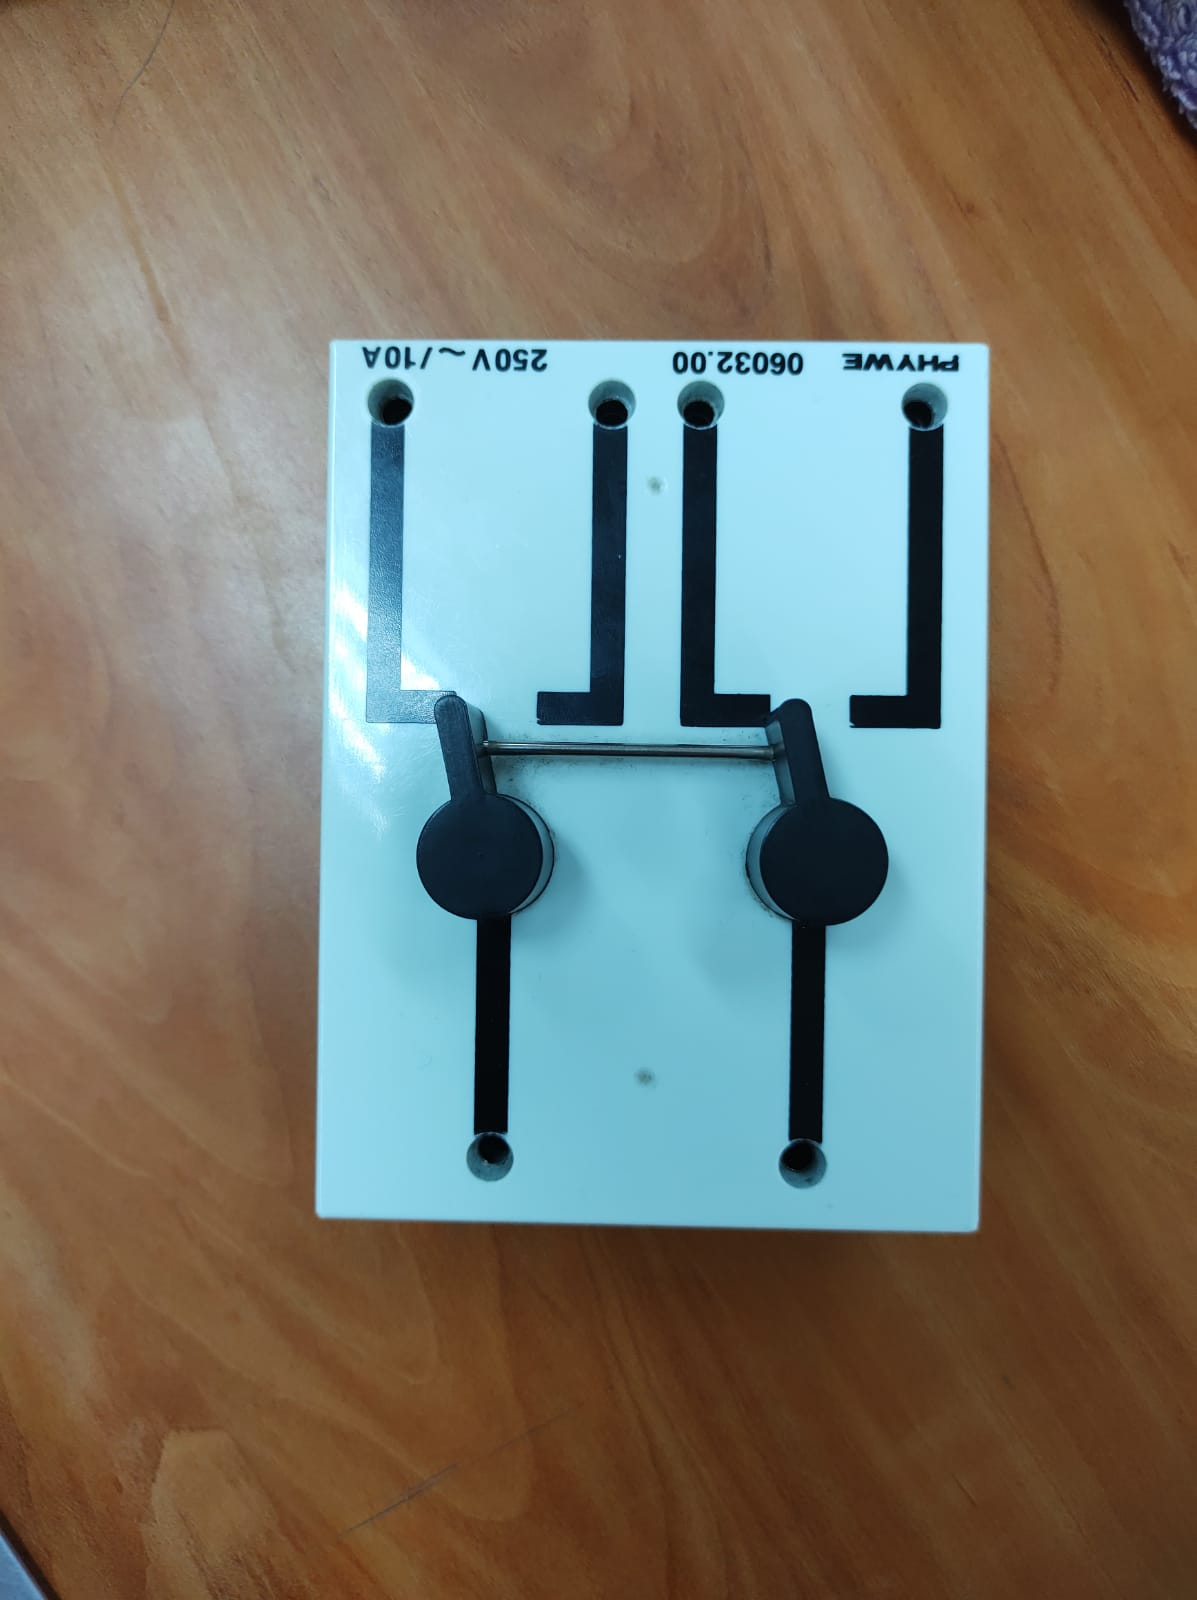
\includegraphics[scale=0.1]{Selector}\\
Reconocimiento del Selector bipolar.
\begin{enumerate}
\item La marca del Selector bipolar es PHYWE.
\item Cuenta con un interuptor bipolar, en el cual podemos cerrar con el interuptor K.
\item Cuenta con una terminal de entrada negativa.
\item Cuenta con una terminal de entrada positiva.
\end{enumerate}
\end{center}

\subsection{Fuente universal.}

Una fuente universal es una fuente de alimentación que puede adaptarse a diferentes tipos de dispositivos eléctricos y electrónicos. Estas fuentes de alimentación suelen tener un amplio rango de voltajes de salida y una selección de conectores para adaptarse a una amplia variedad de dispositivos. Las fuentes de alimentación universales son útiles para viajeros que necesitan cargar diferentes dispositivos en diferentes países, así como para técnicos y profesionales que necesitan una fuente de alimentación que pueda adaptarse a diferentes tipos de equipos.

\begin{center}
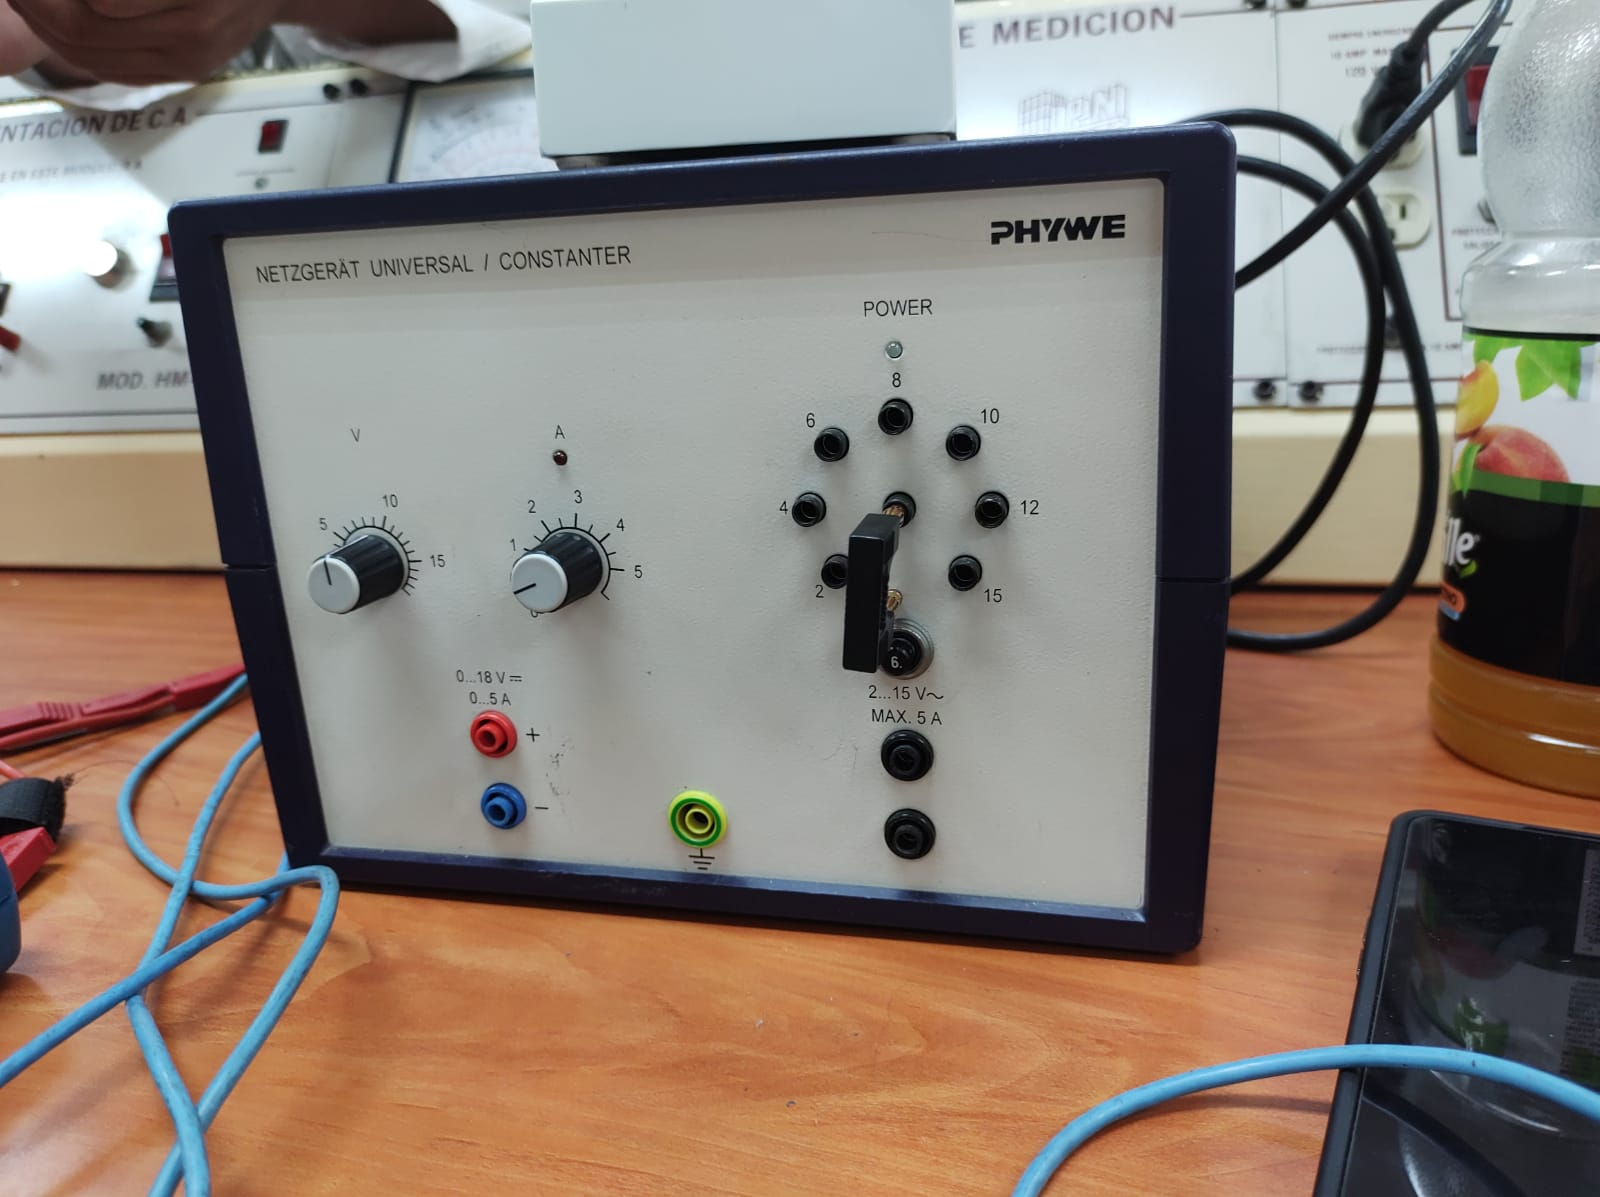
\includegraphics[scale=0.1]{Fuente}\\
Reconocimiento del Fuente universal.
\begin{enumerate}
\item La marca de la fuente universal es PHYWE.
\item Cuenta con 20 posiciones en la perilla V.
\item Cuenta con 6 posiciones en la perilla A.
\item Cuenta con una terminal de entrada negativa de color azul.
\item Cuenta con una terminal de entrada positiva de color roja.
\item Cuenta con un interruptor de encendido y apagado.
\end{enumerate}
\end{center}

\subsection{Amperimetro.} 

Un amperímetro es un instrumento de medición que se utiliza para medir la corriente eléctrica en un circuito eléctrico. La corriente eléctrica se mide en amperios (A), y un amperímetro se conecta en serie en el circuito, es decir, la corriente que se desea medir pasa a través del amperímetro. Los amperímetros pueden ser analógicos o digitales, y su rango de medición se suele indicar en la escala del instrumento o en la pantalla digital. Es importante tener en cuenta que los amperímetros deben ser capaces de soportar la corriente máxima que puede circular por el circuito, de lo contrario se pueden dañar o producir situaciones de peligro. Los amperímetros se utilizan en diversos campos, como la electrónica, la industria eléctrica, la medicina, entre otros. 

\begin{center}
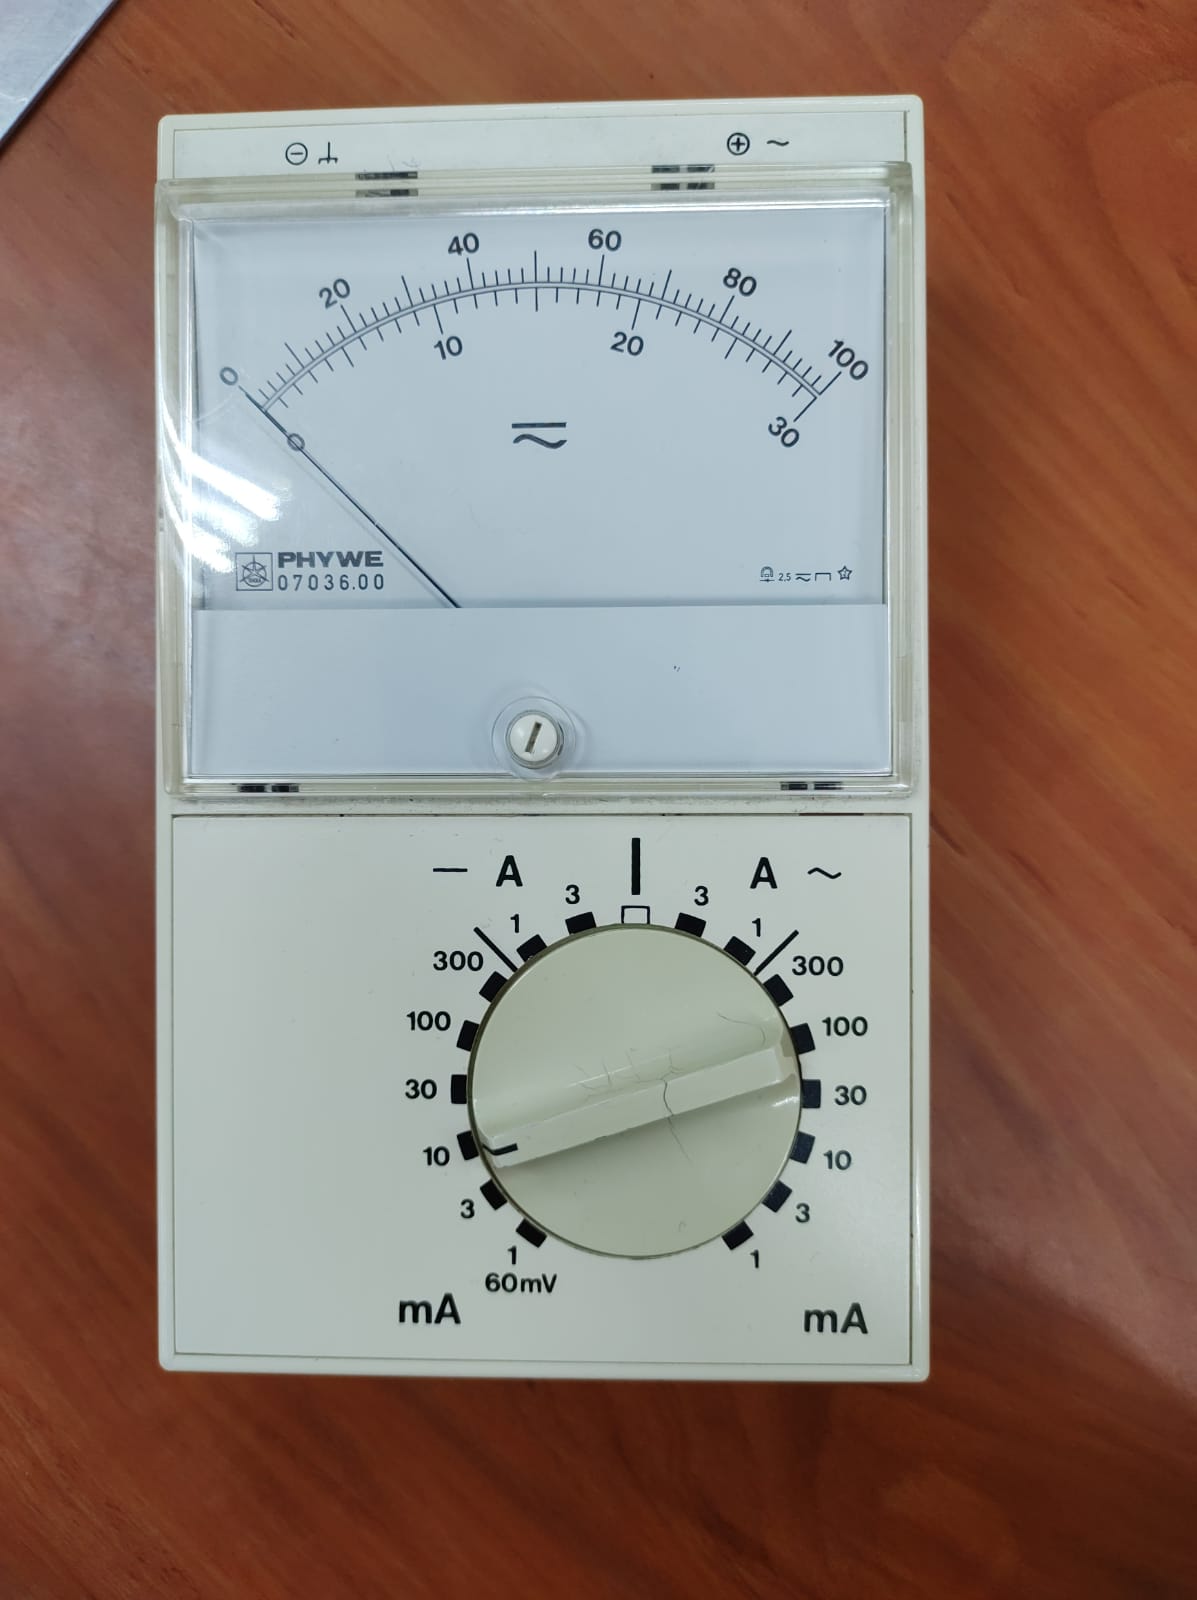
\includegraphics[scale=0.1]{Amperimetro}\\
Reconocimiento del Amperimetro.
\begin{enumerate}
\item La marac de Amperimetro 1-300 mA es PHYWE.
\item Cuenta con una terminal de entrada negativa.
\item Cuenta con una terminal de entrada positiva.
\item Cuenta con 17 posiciones en la perilla mA.
\item El rago de posiciones en -A es de: 1,3,10,30,100,300/1/3.
\item El rago de posiciones en ~A es de: 1,3,10,30,100,300/1/3.
\end{enumerate}
\end{center}

\subsection{Cables de conexión.}

Los cables de conexión son conductores eléctricos que se utilizan para conectar diferentes elementos de un circuito eléctrico, como por ejemplo, dispositivos electrónicos, paneles solares, baterías, etc. Estos cables suelen estar formados por dos conductores eléctricos (denominados positivo y negativo) que van recubiertos por un material aislante para evitar cortocircuitos o contactos involuntarios.

Los cables de conexión pueden tener diferentes grosores o calibres, lo que influirá en su capacidad para soportar corrientes eléctricas de mayor o menor intensidad. También pueden ser de diferentes materiales, como el cobre o el aluminio, dependiendo de las necesidades del circuito.

\begin{center}
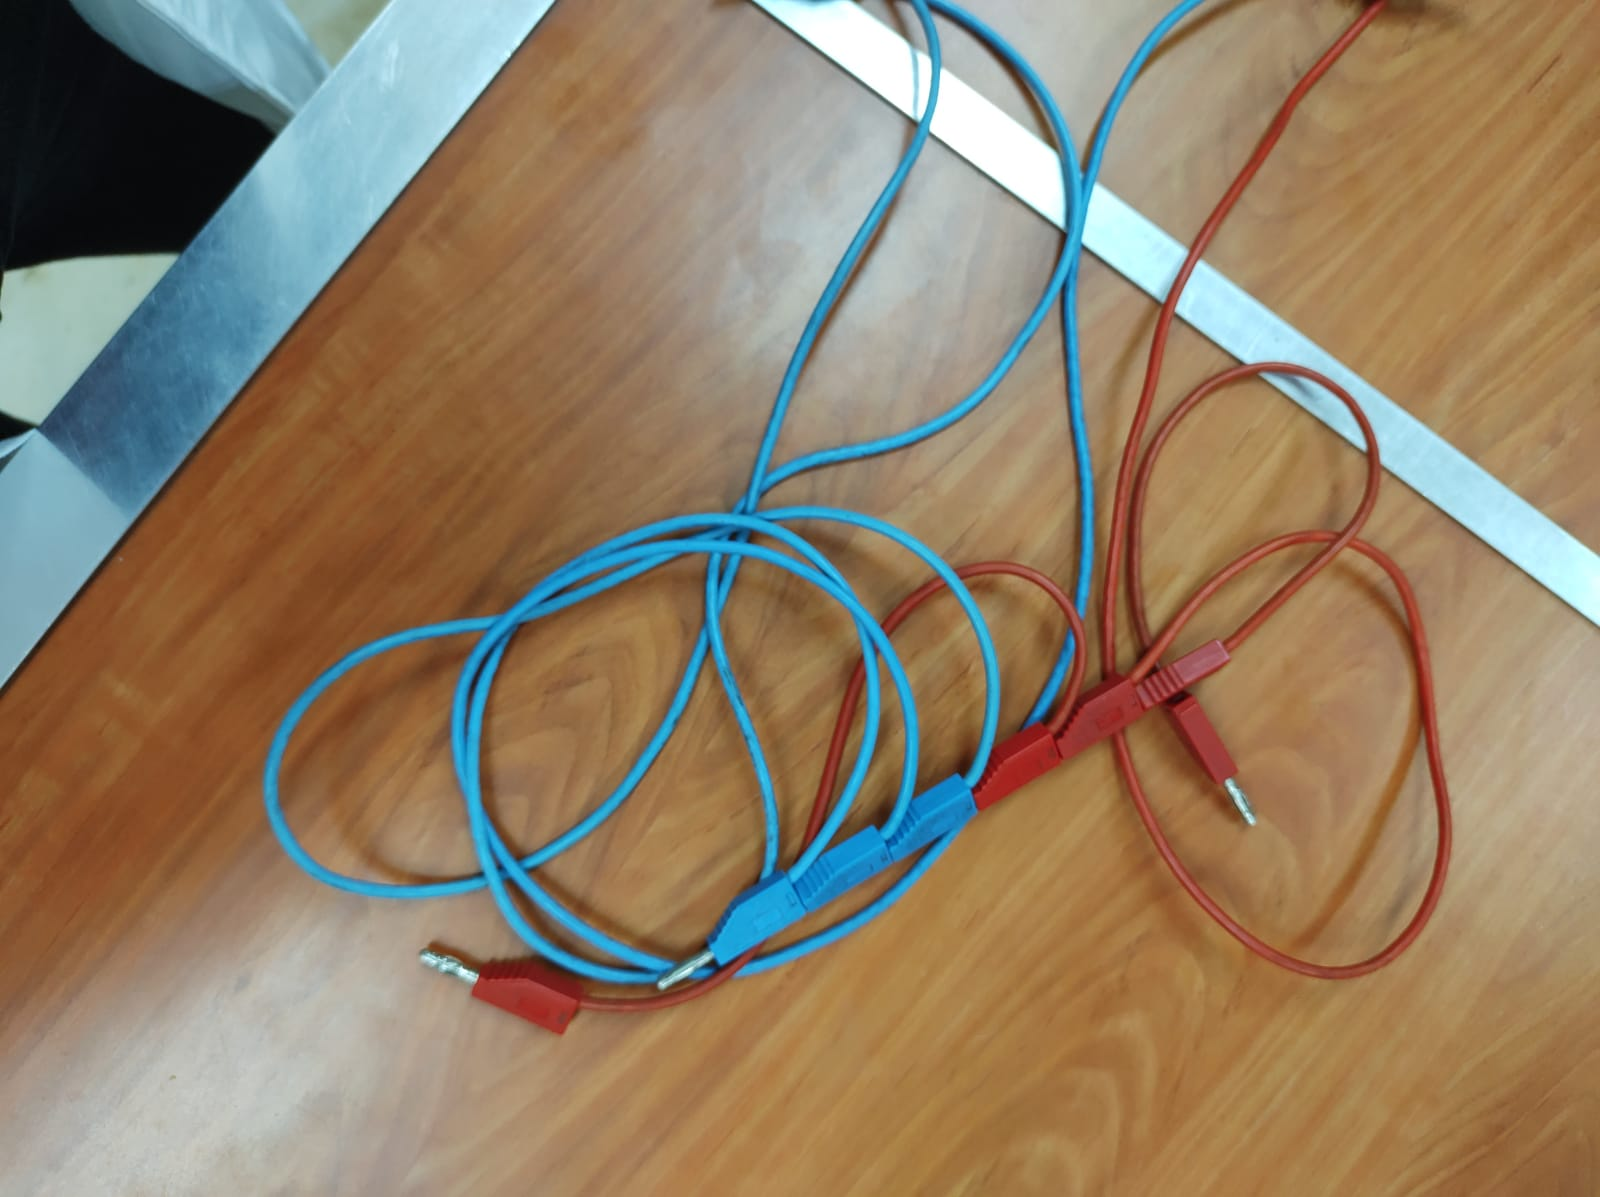
\includegraphics[scale=0.1]{Cables}\\
Reconocimiento del Cables de conexión.
\begin{enumerate}
\item Son 6 cables de conexión.
\item Hay 3 cables de conexión negativa los cuales son de color azul y se conectan en la teminal de entrada negativa.
\item Hay 3 cables de conexión positiva los cuales son de color rojo y se conectan en la teminal de entrada positiva.
\end{enumerate}
\end{center}

\subsection{Década de resistencias.}

Una década de resistencia es un dispositivo de medición utilizado en electrónica para medir valores de resistencia eléctrica con gran precisión. Este dispositivo consiste en una serie de resistores conectados en serie, cada uno con un valor de resistencia específico que se elige girando un dial. Al girar el dial, se selecciona un valor de resistencia específico para medir. Las décadas de resistencia se utilizan comúnmente en laboratorios de electrónica y en la calibración de instrumentos de medición de resistencia eléctrica. Se pueden encontrar décadas de resistencia analógicas y digitales en el mercado. En la actualidad, las décadas de resistencia digitales son más populares debido a su facilidad de uso y mayor precisión.

\begin{center}
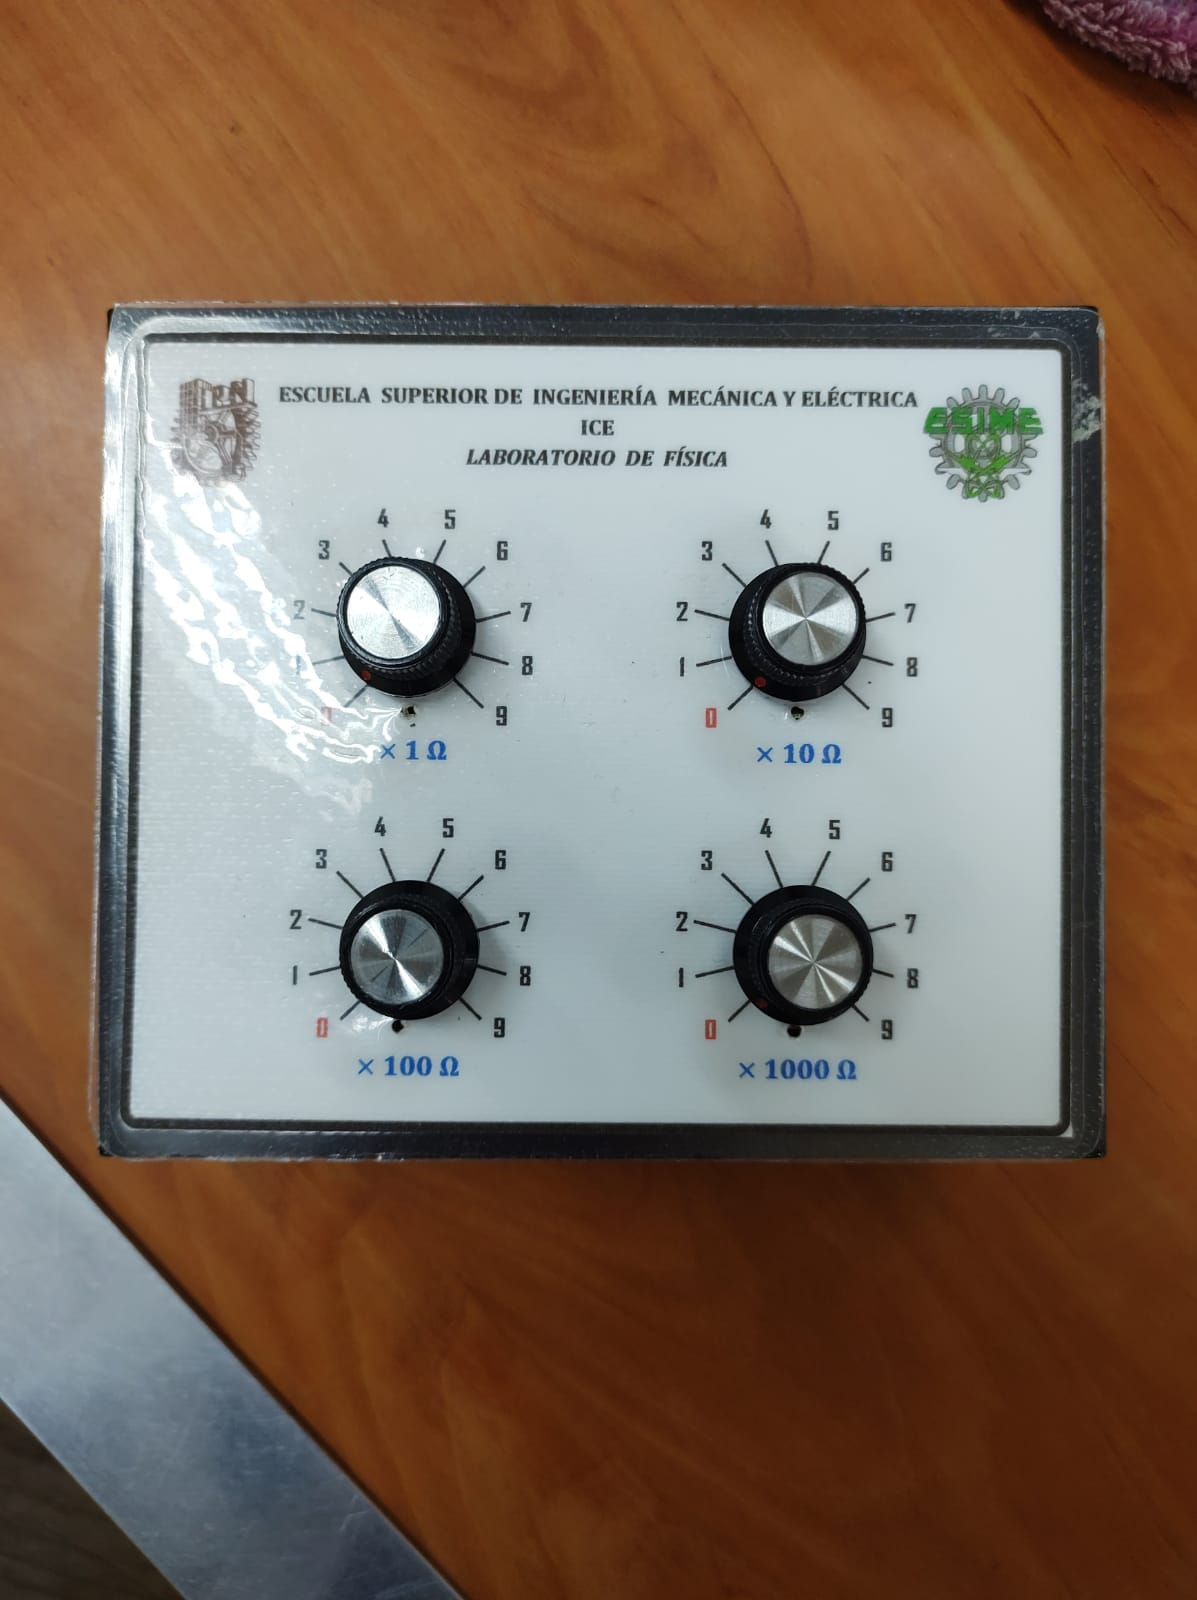
\includegraphics[scale=0.1]{Decada}\\
Reconocimiento del Década de resistencias.
\begin{enumerate}
\item Cuenta con 4 perillas.
\item La primera perilla cuenta con 9 posiciones y esta en X1 Ohmio.
\item La segunda perilla cuenta con 9 posiciones y esta en X10 Ohmios.
\item La tercera perilla cuenta con 9 posiciones y esta en X100 Ohmios.
\item La cuarta perilla cuenta con 9 posiciones y esta en X1000 Ohmios.
\item Cuenta con una terminal de entrada negativa.
\item Cuenta con una terminal de entrada positiva.
\end{enumerate}
\end{center}


\section{Desarrollo experimental.}

1.-Relación entre voltaje y corriente. 
En este primer ejercicio se requirió armar un circuito teniendo precaución de que el selector del medidor este señalado la escala de 3 mA  o mayor y que la escala de voltaje de la fuente no marque más de 15 volts. 
Posterior a esto y después de comprobar que el circuito estaba bien armado, cerramos el interruptor K y con los controles (grueso y fino) de salida de voltaje de la fuente regulada ajustamos el voltaje de acuerdo a los valores indicados en la tabla.
 
2.- Relación entre resistencia y corriente. 
Con el circuito posteriormente armado encendimos la fuente regulada y con ayuda de los controles (grueso y fino) ajustamos el voltaje de salida aplicado al resistor a un valor de 8 volts. 
Realizando lo anterior cerramos el interruptor K y medimos la intensidad de corriente para cada valor de resistencia, (abriendo el interruptor K antes del cambio de resistencia). 

3.- Relación entre voltaje y resistencia 
Con el mismo circuito cerramos el interruptor K y lentamente con ayuda de los controles aumentamos el voltaje aplicando a la resistencia hasta que el amperímetro se obtenga una lectura de 2 Ma, cuando alcanzamos este valor (abrimos el interruptor K incrementando el valor de la resistencia según lo indicado en la tabla



\section{Analisis de resultados}
Relación entre voltaje y corriente 
Tabla1 
El circuito armado el medidor estaba señalando la escala de 3 mA o mayor y que la escala de voltaje de la fuente no marcara más de 15 Volts. 
En los resistores óhmicos la corriente aumenta en la misma proporción que aumenta el diferencial de potencial eléctrico, con una resistencia de 6800Ω
De acuerdo con la gráfica la constante de proporcionalidad entre el voltaje y la corriente es de 0.3Am, esto quiere decir que se puede considerar el resistor como una resistencia óhmica. 

Relación entre resistencia y corriente 
Tabla 2 
Encendiendo la fuente regulada y con ayuda de los controles ajustamos el voltaje de salida aplicando el resistor a un valor de 8 volts, con lo anterior cerramos el interruptor K y medimos la intensidad de corriente. 
La curva que representa la gráfica es decreciente, la relación que existe entre la constante de proporcionalidad de la segunda gráfica y el voltaje aplicado es que entre más voltaje se le ponga a la resistencia, esta misma disminuirá como lo muestra la grafica 

Relación entre voltaje y resistencia 
Tabla 3 
El arreglo del circuito es el mismo que se muestrea anteriormente iniciando con un valor de resistencia R=2000Ω
En esta encerramos el interruptor K y lentamente con ayuda de los controles aumentamos el voltaje a la resistencia hasta que el amperímetro obtuviera una lectura de 2 mA
La relación que existe entre V y R cuando I se mantiene constante es de 2 Am\\
Tabla 1.
\begin{center}
	\begin{adjustbox}{width=245pt}
		\begin{tabular}{|c|c|c|c|c|c|c|c|c|c|}
			\hline
			V(V) & 0 & 2 & 4 & 6 & 8 & 10 & 12 & 14 & 15 \\
			\hline
			I(mA) & 0 & 0.46 & 0.70 & 1.04 & 1.40 & 1.69 & 1.90 & 2.19 & 2.41 \\
			\hline
			
		\end{tabular}
	\end{adjustbox}
\end{center} 
Tabla 2
\begin{center}
	\begin{adjustbox}{width=245pt}
		\begin{tabular}{|c|c|c|c|c|c|c|c|c|}
			\hline
			R(K$\varOmega$) & 3 & 4 & 5 & 6 & 7 & 8 & 9 & 10  \\
			\hline
			I(mA) & 2.60 & 1.97 & 1.58 & 1.32 & 1.13 & 1.00 & 0.89 & 0.88 \\
			\hline
			
		\end{tabular}
	\end{adjustbox}
\end{center}
Tabla 3
\begin{center}
	\begin{adjustbox}{width=245pt}
		\begin{tabular}{|c|c|c|c|c|c|c|c|}
			\hline
			R(K$\omega$) & 2 & 3 & 4 & 5 & 6 & 7 & 8   \\
			\hline
			V(V) & 3 & 5 & 7 & 9 & 11 & 14 & 16 \\
			\hline
			
		\end{tabular}
	\end{adjustbox}
\end{center}


	%----------------------------------------------------------------
	\begin{tikzpicture}
		\begin{axis}[
			title={Grafica 1},
			axis lines = left,
			xlabel = \(V(V)\),
			ylabel = {\(I(mA)\)},
		]
		%Below the red parabola is defined
		\addplot [
			domain=0:15,
			samples=100, 
			color=red,
		]
		{0.00003*x^5 - 0.0012*x^4 + 0.015*x^3 - 0.0821*x^2 + 0.3341*x + 0.0032};
		
		\end{axis}
		\end{tikzpicture}
		%----------------------------------------------------------------
	
		\begin{tikzpicture}
			\begin{axis}[
				title={Grafica 2},
				axis lines = left,
				xlabel = \(R(K\Omega))\),
				ylabel = {\(I(mA)\)},
			]
			%Below the red parabola is defined
			
			%Here the blue parabola is defined
			\addplot [
				domain=0:10, 
				samples=100, 
				color=blue,
				]
				{0.0001*x^6 - 0.004*x^5 + 0.0646*x^4 - 0.5526*x^3 + 2.7255*x^2 - 7.7652*x + 11.96};
			
		
			\end{axis}
			\end{tikzpicture} 
		%----------------------------------------------------------------
		
		\begin{tikzpicture}
			\begin{axis}[
				title={Grafica 3},
				axis lines = left,
				xlabel = \(R(K\Omega)\),
				ylabel = {\(V(V)\)},
			]
			
		
			\addplot [
				domain=0:8, 
				samples=100, 
				color=black,
				]
				{-0.0152*x^4 + 0.303*x^3 - 2.0682*x^2 + 7.7089*x - 6.3571};
			
			\end{axis}
			\end{tikzpicture}

\section{Conclusiones.}

\subsection*{José Emilio Hernández Huerta.}
Durante la práctica, pude verificar que la corriente es directamente proporcional a la tensión aplicada y que disminuye cuando se incrementa la resistencia. Esto me ha enseñado la importancia de elegir los componentes adecuados para garantizar un funcionamiento óptimo del circuito, así como la necesidad de considerar la resistencia al diseñar y analizar circuitos eléctricos. 

\subsection*{Daniela Elizabeth Pérez Vargas.}
En conclusión, la Ley de Ohm establece una relación directa entre la intensidad de corriente que fluye a través de un resistor y la diferencia de potencial aplicada a sus terminales. Esta ley es fundamental para el estudio de la electricidad y es aplicable en una gran variedad de circuitos eléctricos. Asimismo, la ley de Ohm es importante en la resolución de problemas de circuitos eléctricos en la vida real y en el diseño de sistemas eléctricos más eficientes. A través de la experimentación y el análisis de las magnitudes eléctricas.
\subsection*{Jesús Martinez Amac.}
En conclusión, la ley de Ohm establece que la corriente que fluye a través de un conductor es proporcional a la diferencia de potencial aplicada y inversamente proporcional a la resistencia del conductor. Esta ley es muy útil en la comprensión y diseño de circuitos eléctricos, ya que nos permite calcular la cantidad de corriente que fluye en un circuito dado en función de las variables mencionadas. Además, la ley de Ohm es uno de los primeros y más importantes conceptos en la electrónica y es esencial para el estudio de temas más avanzados en el campo.

\subsection*{Nataly Bejarano Garduño.}
El “voltaje” o Diferencial de potencial eléctrico, es el trabajo por unidad de carga eléctrica que ejerce sobre una partícula un campo eléctrico. La resistencia es una medida de la oposición al flujo de corriente en un circuito eléctrico La corriente eléctrica es el flujo de carga eléctrica que atraviesa un material conductor durante un periodo de tiempo determinado. 
La relación entre corriente, voltaje y resistencia se expresa por la ley de Ohn. Determina que la corriente que fluye en un circuito es proporcionar directamente al voltaje aplicado e inversamente proporcional a la resistencia del circuito, y aunque son parecidas no son lo mismo, aunque si se complementan.

\subsection*{Uriel Grimaldi Díaz.}
En conclusión el diferencial de potencial eléctrico, la carga eléctrica y la resistencia son conceptos muy diferentes pero que se complementan entre si, en el circuito eléctrico, el suministro de potencia genera una presión eléctrica, el amperímetro es equivalente al medidor de flujo y el voltimetro mide la diferencia de presión eléctrica.

\begin{thebibliography}{0}
	\bibitem{citekey}[Ley de Ohm . (2021, 1 de marzo). Portal Académico Del CCH.]
	\bibitem{citekey}[La ley de Ohm - Electricidad y electrónica - Picuino . (Dakota del Norte)]
		
\end{thebibliography}

\end{multicols}

\end{document}
